\documentclass[a4paper, 11pt]{report}
\usepackage{setspace}
\setstretch{1,15}
%\usepackage{newunicodechar}
\usepackage[french]{babel}
\usepackage{graphicx}
\graphicspath{{images/}}
\usepackage{fontspec}
\setmainfont{Verdana}
\usepackage{lipsum}
\renewcommand{\thesection}{\arabic{section}}
\usepackage{ulem}
\usepackage{geometry}
\geometry{hmargin=2.5cm,vmargin=3.5cm}
\usepackage{fancyhdr}

\author{JUILLIARD-COGNE}


%%exemple titre : Un semestre à cracovie:
%% Entre orient et occident
%%De l'autre coté du rideau de fer
%%Associé à l'Est, veut se rapprocher de l'Ouest


\begin{document}

\pagestyle{fancy}

\fancyhead{}\fancyfoot{}
%\fancyhead[ER]{Projet SALE} Fonctionne que si en mode book
%\fancyhead[ER]{L3 informatique Reims Année 2022-2023} Fonctionne que si en mode book

\fancyhead[L]{JUILLIARD Quentin - COGNE Romain} 
\fancyhead[R]{\thepage} 
\fancyfoot[R]{Année Universitaire 2022 - 2023}

\begin{title}

\title{
    {\Huge Le système d'achat de l'energie}\\
    \vspace{1 cm}
    {\LARGE JUILLIARD Quentin S5O6}\\
    {\LARGE COGNE Romain S5O6}\\
    \vspace{2.5 cm}
    {
\includegraphics[width=80mm, height=40mm]{logo_univ}}\\
    \vspace{2.5 cm}
    {\Large Monsieur BOISSON, INFO0503 / Département Informatique}\\
    \vspace{1 cm}
    {\date{\Large Dimanche 11 décembre 2022}}}
\end{title}

\maketitle
\tableofcontents
\clearpage

%\pagenumbering{arabic}

\section{Introduction}


\newpage

\section{Lancement du projet}
Voyons désormais comment démarrer le projet.


\subsection{Organisation des fichiers}
Dans notre archive, une fois décompressé, vous trouverez de nombreux dossiers et fichiers.
\begin{itemize}
    \item Le dossier ".vscode" si vous êtes sous windows et que vous utilisez le logiciel Visual Studio Code comme nous, ce dossier apparaîtra. Il contient le fichier "Launch.json" , et nous reviendrons dessus dans la sous-partie "Compilation Windows".
    \item   Le dossier "cls", vous retrouverez l'ensemble des ".class" issue de la compilation JAVA.
    \item   Le dossier "doc" regroupe l'ensemble de la documentation de notre projet. Ce dossier n'est pas réellement utile car nous n'avons pas réalisé de documentation présise à l'interieur de notre projet par manque de temps. Nous avons commenté directement dans notre code sans utiliser les options et la syntaxe de la java doc.
    \item   Le dossier "lib" contient les librairies qui sont nécessaires pour notre projet. Dans ce projet, nous avons uniquement utilisé la librairie JSON, intitulé ici "json-20220924.jar".
    \item Le dossier "Rapport" contient l'ensemble des fichiers ".tex" du rapport que vous êtes en train de lire, car, en effet le rapport à été realisé sous LaTEX.
    \item Le dossier "src" contient l'ensemble des fichier sources ".java". Dans ce dossier, il existe un sous-dossier pour chaque entité présente dans notre modélisation qui seront exposés dans le Chapitre 4. Il y a également la présence d'un fichier "Lanceur.java" celui-ci sert à lancer l'ensemble des serveur java en multi-threadé en un seul lancement pour plus de simplicité. 
    \item De plus, dans le dossier "src", il existe le dossier "revendeur", le contenu de celui-ci doit être mis dans un serveur WEB PHP comme par exemple wamp ou autre.
    \item Le fichier "commande.txt" regroupe les commandes utiles pour la compilation et le lancement du projet.
     \item Le fichier "config.json" regroupe l'ensemble des ports et adresse des différents serveurs, il seront utilisés par le lanceur pour créer les différentes entités.

\end{itemize}

\newpage

\subsection{Compilation sous Linux}
Si vous travaillez sur un système d'exploitation sous Linux, nous allons vous expliquer dans cette partie comment compiler et lancer le projet.

Tout d'abord, positionnez-vous dans le dossier "Projet-INFO0503" comme ceci : 

\begin{figure}[h]
    \centering
    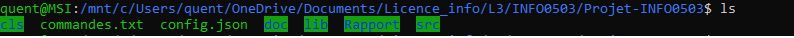
\includegraphics[width= 170mm, height=10mm]{images/positionnement.png}
    \caption{Positionnement dans le dossier}
    \label{img:mesh1}
\end{figure}

Puis réaliser la compilation de l'ensemble des fichiers en utilisant la commande suivante : \newline
\textbf{javac -d cls/ -cp lib/json-20220924.jar -sourcepath src/ src/Lanceur.java}

\begin{figure}[h]
    \centering
    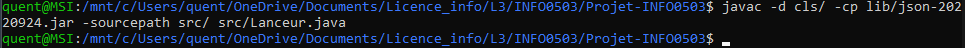
\includegraphics[width= 170mm, height=10mm]{images/compilation.png}
    \caption{Succès de la compilation}
    \label{img:mesh2}
\end{figure}

Une fois la compilation terminée, vous pouvez donc lancer le projet en utilisant la commande suivante : \newline
\textbf{java -cp cls/:lib/json-20220924.jar Lanceur config.json} \newline
Il se peut que vous ayez un message d'erreur comme vous pouvez le voir sur la figure ci-dessous au moment du lancement de vos serveur HTTP.
\begin{figure}[h]
    \centering
    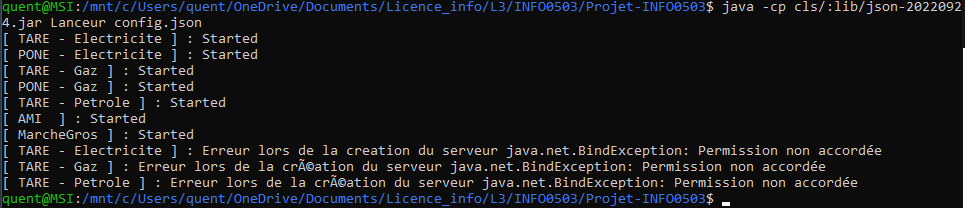
\includegraphics[width= 170mm, height=40mm]{images/erreurLancement.png}
    \caption{Erreur de lancement}
    \label{img:mesh3}
\end{figure}
\newpage
Pour résoudre ce probléme, il vous suffit de passer en superadmin en utilsant le préfixe \textbf{sudo}, comme ceci : \newline
\textbf{sudo java -cp cls/:lib/json-20220924.jar Lanceur config.json}
\begin{figure}[h]
    \centering
    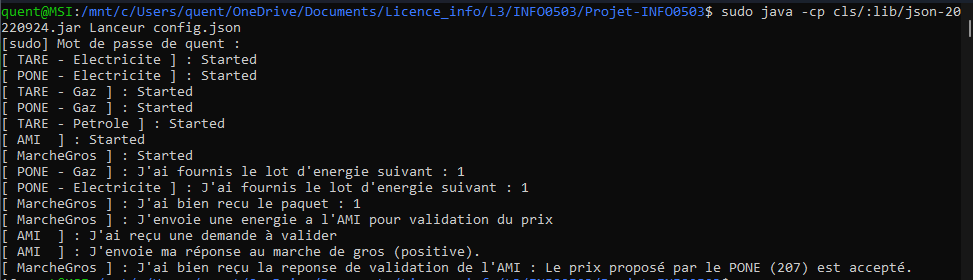
\includegraphics[width= 170mm, height=60mm]{images/succesLancement.png}
    \caption{Succès du lancement}
    \label{img:mesh4}
\end{figure}

Nous voila avec le projet opérationnel du côté serveur. Si le serveur PHP est également opérationnel, vous avez juste à vous rendre dans votre nativateur web et rentrer \textbf{localhost} dans la barre de recherche. Vous pouvez commencer à faire vos simulations d'achat d'énergie, et en même temps consulter les différentes communications entre toutes les entités dans le terminal. Vous pouvez alors essayer les différents sénarios ainsi que créer vos propres commandes.
\begin{figure}[h]
    \centering
    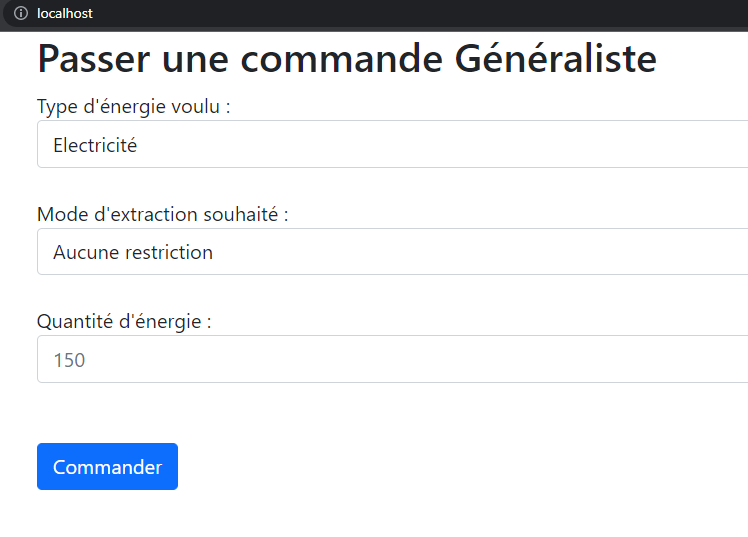
\includegraphics[width= 85mm, height=60mm]{images/Localhost.png}
    \caption{Interface WEB}
    \label{img:mesh5}
\end{figure}
\newpage

\subsection{Compilation sous Windows}
La compilation sous windows est bien plus simple. Pour ce faire vous pouvez utiliser Visual Studio Code ( VS Code) par exemple. \\

Il vous faut ouvrir VS Code puis faire Fichier => Ouvrir Dossier => puis sélectionner le dossier racine du projet comme ci-dessous => puis faire \textbf{Sélectionner un dossier}.
\begin{figure}[h]
    \centering
    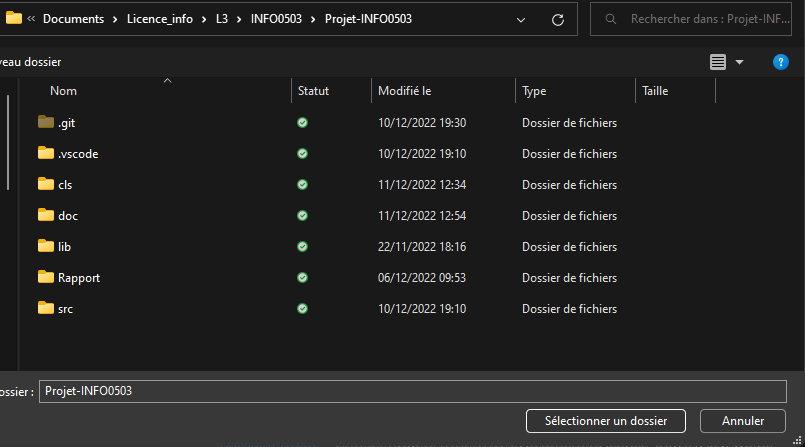
\includegraphics[width= 150mm, height=75mm]{images/FichierASelectionner.png}
    \caption{Dossier à selctionner}
    \label{img:mesh6}
\end{figure}


Une fois le projet ouvert vous pourrez voir sur la gauche de l'interface de VS Code, l'ensemble des dossiers et sous-dossiers contenant les fichiers ".java" du projet, soit l'arborescence du projet.

Une fois que VS Code a reconnu le projet JAVA. Rendez-vous dans le fichier "Lanceur.java", puis dirigez vous à la ligne 28, vous y trouverez un bouton \textbf{Run | Debug} comme sur la figrue suivante.
\begin{figure}[h]
    \centering
    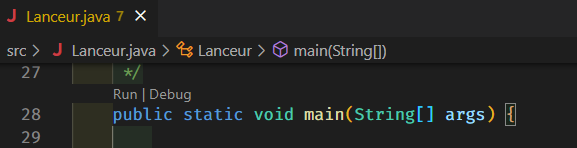
\includegraphics[width= 80mm, height=30mm]{images/BoutonRunDebug.png}
    \caption{Bouton Run | Rebug}
    \label{img:mesh7}
\end{figure}

Il vous suffit de presser le bouton \textbf{Run}, à ce moment là le terminal VS Code se lance mais une erreur apparait comme sur la figure suivante.

\begin{figure}[h]
    \centering
    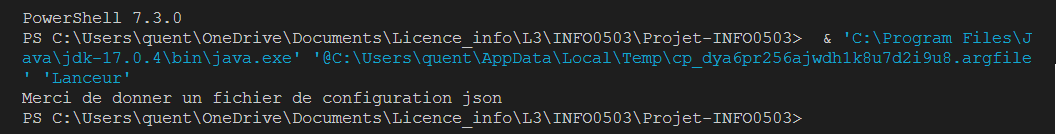
\includegraphics[width= 139mm, height=17mm]{images/ErreurVSCODE.png}
    \caption{Erreur de compilation VSCode}
    \label{img:mesh8}
\end{figure}

Pour résoudre ce problème, il vous suffit de vous rendre dans votre dossier ".vscode" puis dans le fichier 'launch.json" et d'ajouter dans "projectName" la ligne suivante : "args":"config.json" comme sur la figure suivante.

\begin{figure}[h]
    \centering
    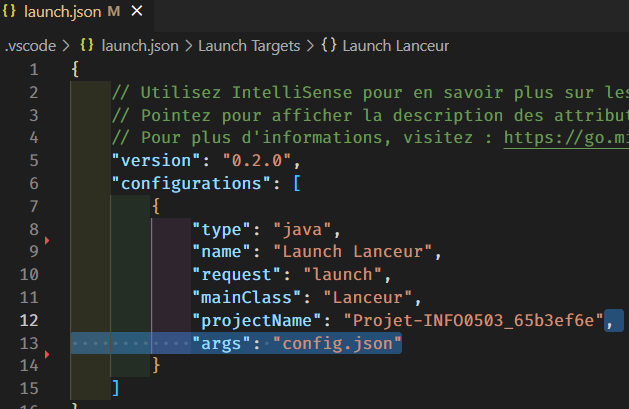
\includegraphics[width= 83mm, height=54mm]{images/lauchjson.png}
    \caption{Ajout de "args"}
    \label{img:mesh9}
\end{figure}

Une fois cette ligne ajoutée, vous pouvez relancer avec le bouton \textbf{Run} et vos serveurs seront opérationnels.
\begin{figure}[h]
    \centering
    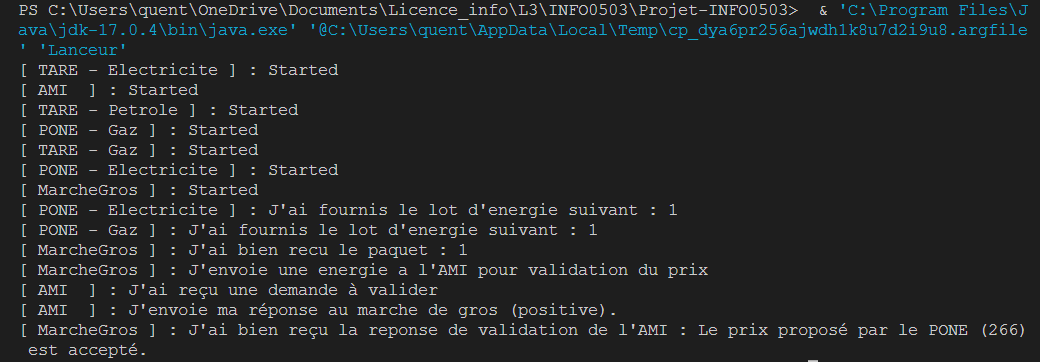
\includegraphics[width= 137mm, height=43mm]{images/VScodeProject.png}
    \caption{Lancement du serveur}
    \label{img:mesh10}
\end{figure}

\newpage

\section{Technologie de communication}

\subsection{Hypertext Transfer Protocol}
\newpage

\subsection{User Datagram Protocol}
\newpage

\subsection{Transmission Control Protocol}
\newpage

\section{Les différentes relations}
\newpage

\subsection{Relation entre Revendeur et Tare}
La relation entre Revendeur et TARE est une relation Hyper Text Protocol (HTTP). La relation HTTP exécute une requête en Transmission Control Protocol (TCP) /IP. L'utilisation de TCP oblige d'avoir un système en d'aquittement. Cette relation peut se modéliser comme ceci :
\\[2cm]
\begin{figure}[h]
    \centering
    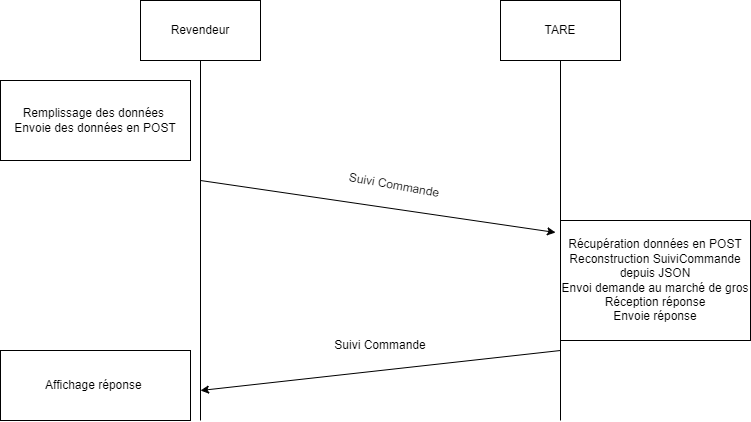
\includegraphics[width=150mm, height=84mm]{images/RevendeurTARE.png}
    \caption{Modélisation de la relation entre Revendeur et TARE}
    \label{img:mesh17}
\end{figure}
\newpage

\subsection{Relation entre Tare et Marché de Gros}
Le Marché de Gros et les TAREs communique entre eux à l'aide du communication UDP. Les informations qui transitent dans les requêtes sont des éléments de type SuiviCommande qui intègrent les variables de type "Energie". Voici à quoi ressemble un échange :

\begin{figure}[h]
    \centering
    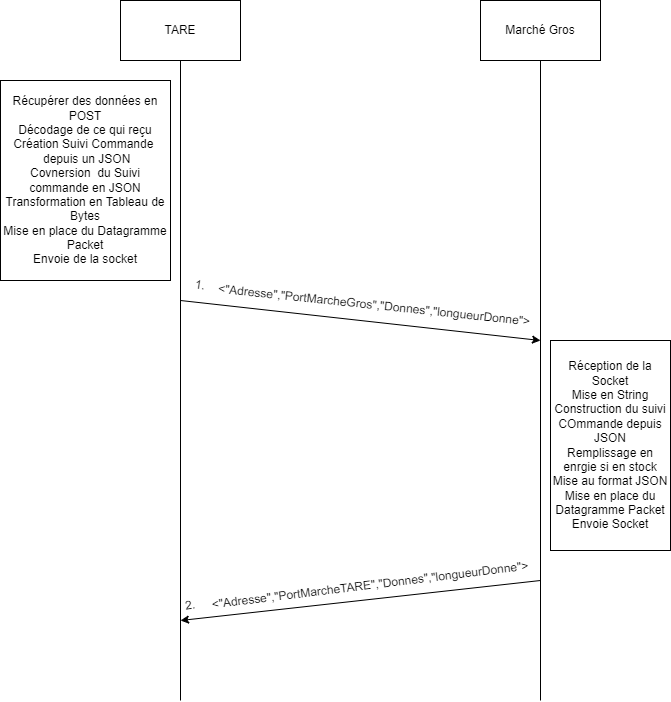
\includegraphics[width=140mm, height=120mm]{images/TAREMG.png}
    \caption{Modélisation de la relation entre Marché de Gros et PONE}
    \label{img:mesh19}
\end{figure}
\newpage

\subsection{Relation entre Marché de Gros et PONE}
Il existe une relation entre le Marché de Gros et le (ou les) PONE. Cette relation est unidirectionnel en User Datagramme Packet ( UDP ), nous envoyons des datagrammes packets du Pone contenant une énergie qui est caractérisée par :
\\
\begin{itemize}
    \item Un type d'energie,
    \item Une quantité envoyé,
    \item Un mode d'extraction,
    \item Un prix unitaire,
    \item Un numéro de lot
    \\
\end{itemize}
 Cette énergie est donc envoyée vers les marché de gros sans vérification d'aquisition car l'UDP est un protocole de transite d'informations sur internet qui n'est pas en capacité de garantir la bonne récéption des informations chez le client.
\begin{figure}[h]
    \centering
    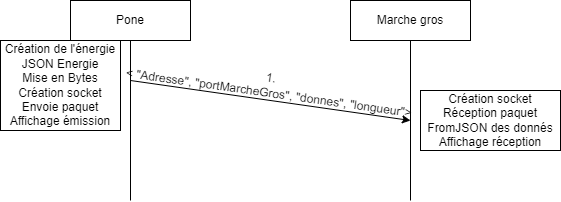
\includegraphics[width=120mm, height=45mm]{images/PONEMG.png}
    \caption{Modélisation de la relation entre Marché de Gros et PONE}
    \label{img:mesh16}
\end{figure}


\subsection{Role de l'AMI}
Dans ce réseau l'AMI ne communique uniquement avec le marché de gros en TCP. Il a pour rôle de vérifier le prix des énergies fournis par les PONE ainsi que de valider la vente avec les TAREs. De plus, l'ensemble des échanges sont sécurisés par un chiffrement RSA pour les crypter. 

Cependant l'AMI doit également certifier, signer les énergies à la sortie de leur production, on parle alors de CeRtificAt D'Origine (ou CRADO). Il doit également certifier, signer les achats, on parle alors de CeRtificAt d'aCHAt (ou CRACHA).
\newpage

\section{Scénarios}

Dans ce projet, il nous a été demandé de réaliser différents scénarios de test.
Il y a en tout 5 scénarios à réaliser.
Nous détaillerons dans les sous-parties suivantes l'ensemble des scénarios, comment nous les avons traités et s'ils sont opérationels ou non, avec les explications si ceux-ci n'ont pas été implémentés.

\subsection{Scénario A}
Dans un système ayant un seul PONE et un seul TARE (en plus du revendeur, du marché de gros et de l'AMI), le client demande une quantité d'énergie sans aucune contrainte particulière et sa demande est toute de suite satisfaite car le PONE produit exactement le type d'énergie demandé. Il y a donc achat (avec enregistrement de l'achat côté AMI) puis distribution au revendeur (en passant par le TARE).
Pour des soucis de simplicité au vue de notre modélisation, nous avons fais le choix
de requêter directement sur notre marché de gros qui est alimenté en permance et automatiquement par nos différents PONEs.
\\[1cm]
Lorsque le bouton "Scénario A" est actionné, nous requêtons notre marché de gros en lui demandant une énegie électrique quelque soit
son mode de production. Dans la requête du "Scénario A", nous passons dans la requête une demande qui est intiulée "Suivi commande". La demande d'énergie souhaitée est une énergie de type "électricité" avec un type d'extraction "Sans restriction" de plus nous passons une quantité égale à 1 pour être sur que celle-ci soit aboutie sans échec.

Il se peut que l'énergie envoyée soit du nucléaire ou du charbon ou encore eolien.

\begin{figure}[h]
    \centering
    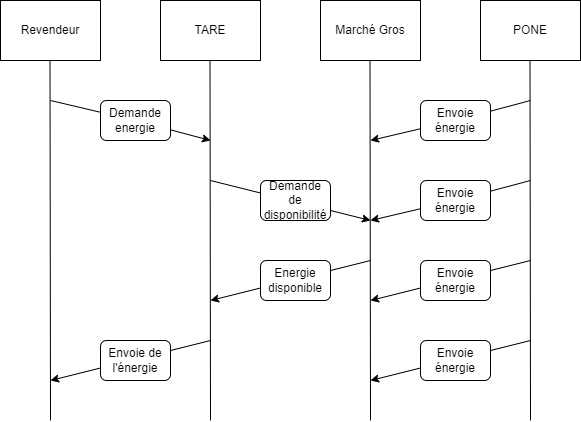
\includegraphics[width=100mm, height=73mm]{images/ScenarioA.png}
    \caption{Schéma du scénario A}
    \label{img:mesh21}
\end{figure}

\newpage


\subsection{Scénario B}
Dans un système ayant un seul PONE et un seul TARE (en plus du revendeur, du marché de gros et de l'AMI), le client demande une quantité d'énergie qui n'est pas disponible pour le moment ... Par contre, au bout de quelques instants de fonctionnement, la demande du client peut-être satisfaite (car le PONE a suffisamment fourni d'énergie). Cela est possible après une nouvelle demande cu client.

Pour ce scénario, nous avons réalisé une demande du client sur une énergie de type "Electricité" avec aucune restriction sur le type d'électricité demandé avec une quantité de 100. La première fois cela échouera, mais après un petit moment, la requête sera satisfaite.

\begin{figure}[h]
    \centering
    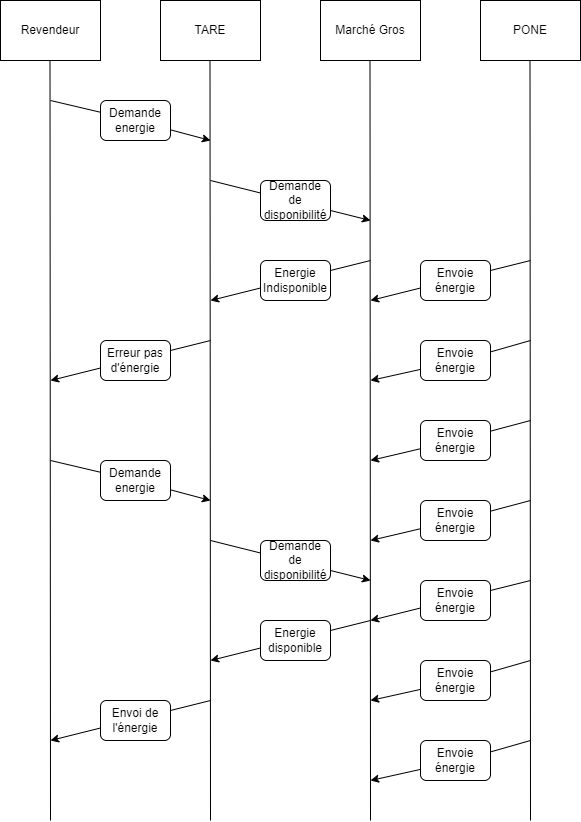
\includegraphics[width=110mm, height=150mm]{images/ScenarioB.png}
    \caption{Schéma du scénario B}
    \label{img:mesh23}
\end{figure}
\newpage

\subsection{Scénario C}
Dans un système ayant un seul PONE et un seul TARE (en plus du revendeur, du marché de gros et de l'AMI), la demande du client ne peut être satisfaite à cause d'une contrainte que le PONE ne peut satisfaire. Par contre, pendant que le système fonctionne, un PONE est rajouté et il peut fournir l'énergie demandée (en une seule production ou au bout d'un certain nombre de production). L'achat d'énergie devient possible et le reste du déroulement respecte le modèle classique.

Dans notre projet, nous démarrons un PONE 30 secondes aprés le démarrage du lanceur. Ce PONE qui est le PONE pétrole va alors envoyer de l'energie au marché de gros tous comme les autres PONE.
Dans notre projet, pour être sur que celle-ci soit satisfaite dés la 1ère demande (une fois le PONE en marche), nous avons décidé de demander au revendeur du Pétrole mais sans type d'extraction précise avec une quantité de 1.


\begin{figure}[h]
    \centering
    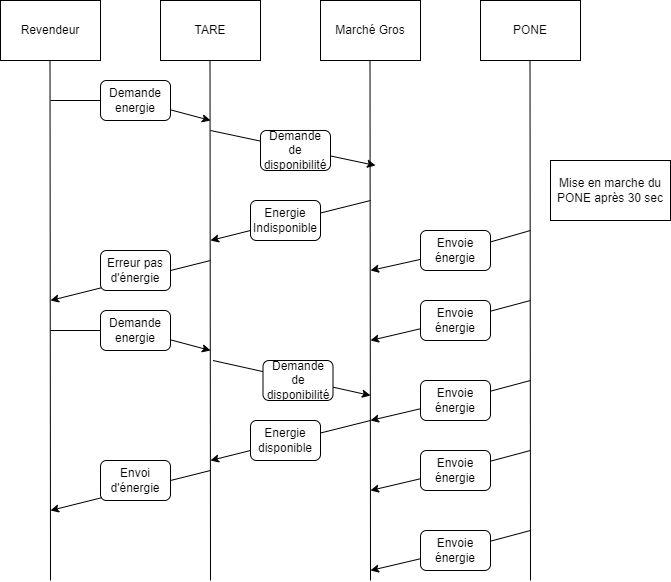
\includegraphics[width=134mm, height=116mm]{images/ScenarioC.png}
    \caption{Schéma du scénario C}
    \label{img:mesh24}
\end{figure}
\newpage

\subsection{Scénario D}
Dans un système ayant deux PONEs et deux TAREs (en plus du revendeur, du marché de gros et de l'AMI), pour être satisfaite rapidement, la demande du client doit se baser sur la sommes des énergies fournies par les 2 PONEs. Par contre, les TAREs ne peuvent acheter qu'à un seul lot d'énergie d'un PONE à la fois (via le marché de gros). C'est donc le revendeur qui doit gérer le rassemblement des 2 retours de TARE pour construire la réponse au client.
\\[1cm]
Ce scénario n'a pas été réalisé dans notre projet par manque de temps car nous devions réaliser des modifications importantes dans notre code et finir le rapport, nous avons pris la décision de ne pas le faire.
Cependant nous avons quand même réfléchi à celui-ci et comment nous l'aurions implémenté si nous avions eu le temps.

\begin{figure}[h]
    \centering
    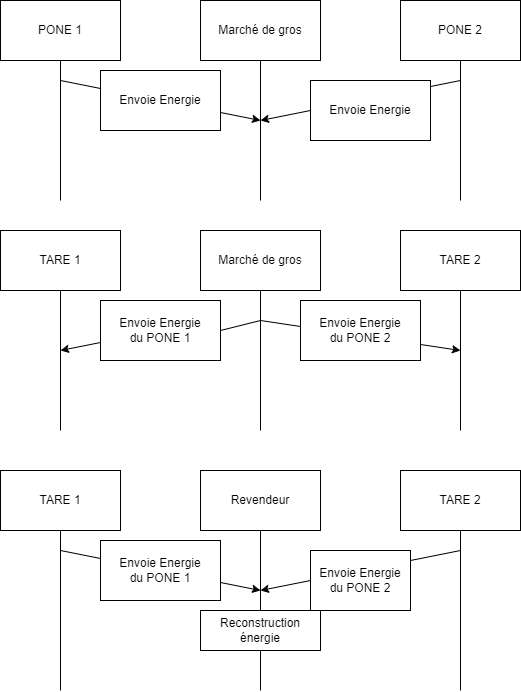
\includegraphics[width=110mm, height=140mm]{images/ScenarioD.png}
    \caption{Schéma du scénario D}
    \label{img:mesh25}
\end{figure}
\newpage

\subsection{Scénario A2}
Il s'agit du scénario A dans lequel, à la fin de l'achat de l'énergie, le client demande à faire vérifier le numéro de suivi de l'énergie achetée. Cela signifie qu'il faut valider le CRACHA et le CRADO qu'il contient auprès de l'AMI qui est l'autorité de certification.
\\[1cm]
 Ce scénario n'a pas été traité dans notre projet, mais voici à quoi cela aurait du ressemblé :
\\
 \begin{figure}[h]
    \centering
    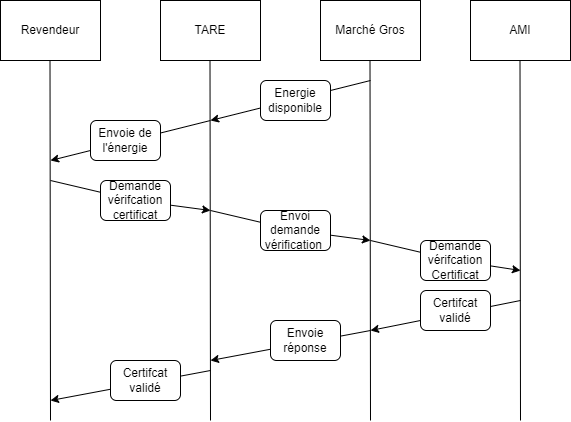
\includegraphics[width=130mm, height=100mm]{images/ScenarioA2.png}
    \caption{Schéma du scénario A2}
    \label{img:mesh22}
\end{figure}
\newpage

\section{Conclusion}
\newpage

\listoffigures
%\listoftables
+

\end{document}
